%Authors guidlines: http://royalsocietypublishing.org/instructions-authors
% 2500 words max (includes the title page, abstract, references, acknowledgements and figure/table legends)
% current version is around 3700. I think a big cut down can be done on the references.
% We allow a maximum of 4 displays, only 2 of which can be figures.

\documentclass[12pt,letterpaper]{article}


%Packages
\usepackage{pdflscape}
\usepackage{fixltx2e}
\usepackage{textcomp}
\usepackage{fullpage}
\usepackage{float}
\usepackage{latexsym}
\usepackage{url}
\usepackage{epsfig}
\usepackage{graphicx}
\usepackage{amssymb}
\usepackage{amsmath}
\usepackage{bm}
\usepackage{array}
\usepackage[version=3]{mhchem}
\usepackage{ifthen}
\usepackage{caption}
\usepackage{hyperref}
\usepackage{amsthm}
\usepackage{amstext}
\usepackage{enumerate}
\usepackage[osf]{mathpazo}
\usepackage{dcolumn}
\usepackage{lineno}
\usepackage{longtable}
\pagenumbering{arabic}

\newcolumntype{L}[1]{>{\raggedright\let\newline\\\arraybackslash\hspace{0pt}}m{#1}}
\newcolumntype{C}[1]{>{\centering\let\newline\\\arraybackslash\hspace{0pt}}m{#1}}
\newcolumntype{R}[1]{>{\raggedleft\let\newline\\\arraybackslash\hspace{0pt}}m{#1}}

%Pagination style and stuff % NC: Note that these are all syst biol specific.
\linespread{2}
\raggedright
\setlength{\parindent}{0.5in}
\setcounter{secnumdepth}{0} 
\renewcommand{\section}[1]{%
\bigskip
\begin{center}
\begin{Large}
\normalfont\scshape #1
\medskip
\end{Large}
\end{center}}
\renewcommand{\subsection}[1]{%
\bigskip
\begin{center}
\begin{large}
\normalfont\itshape #1
\end{large}
\end{center}}
\renewcommand{\subsubsection}[1]{%
\vspace{2ex}
\noindent
\textit{#1.}---}
\renewcommand{\tableofcontents}{}
%\bibpunct{(}{)}{;}{a}{}{,}

%---------------------------------------------
%
%       START
%
%---------------------------------------------

\begin{document}


\newcommand{\beginsupplement}{%
    \setcounter{table}{0}
    \renewcommand{\thetable}{S\arabic{table}}%
    \setcounter{figure}{0}
    \renewcommand{\thefigure}{S\arabic{figure}}%
}

%Running head
\begin{flushright}
Version dated: \today
\end{flushright}

\bigskip
\medskip
\begin{center}

\noindent{\Large \bf Assessment of available anatomical characters for linking living mammals to fossil taxa in phylogenetic analyses}

\bigskip
\noindent{\Large \bf Electronic Supplementary Material 1}

\bigskip
\noindent {\normalsize \sc Thomas Guillerme$^1$$^,$$^*$ and Natalie Cooper$^1$$^,$$^2$}\\
\noindent {\small \it 
$^1$School of Natural Sciences, Trinity College Dublin, Dublin 2, Ireland.\\
$^2$Department of Life Sciences, Natural History Museum, Cromwell Road, London, SW7 5BD, UK.}\\
\medskip
\noindent{*\bf Corresponding author.} \textit{t.guillerme@imperial.ac.uk}\\  
\vspace{1in}

\end{center}

\newpage






% TO DO!
% NC: It's important to follow up on typo and grammar issues in the supp for things that were mentioned in the main text. For example, dropping https... MorphoBank...









\section{1 - Data collection}
\subsection{Public repositories}
We downloaded available matrices containing fossil and/or living mammal taxa from the three databases using the following list of keywords:

\texttt{Mammalia; Monotremata; Marsupialia; Placentalia; Macroscelidea; Afrosoricida; Tubulidentata; Hyracoidea; Proboscidea; Sirenia; Pilosa; Cingulata; Scandentia; Dermoptera; Primates; Lagomorpha; Rodentia; Erinaceomorpha; Soricomorpha; Cetacea; Artiodactyla; Cetartiodactyla; Chiroptera; Perissodactyla; Pholidota; Carnivora; Didelphimorphia; Paucituberculata; Microbiotheria; Dasyuromorphia; Peramelemorphia; Notoryctemorphia; Diprotodontia}.

Details about the specific search options used for each public repository are listed below.
Note that some matrices were downloaded from more than one database but this is not a problem because we are interested in the total number of unique living operational taxonomic units (OTUs), therefore even if some were present in more than one matrix they still only counted as a single OTU.

\subsubsection{MorphoBank}
We accessed the MorphoBank repository (\url{morphobank.org}) on 10th June 2015 and used the keywords listed above in the search menu.
We downloaded the data associated with each project matching with the keyword.

\subsubsection{Graeme Lloyd}
We accessed Graeme Lloyd's website repository (\url{graemetlloyd.com/}) on 10th June 2015 and downloaded all the matrices that were available with a direct download link in the mammal data section of the website (\texttt{graemetlloyd.com/matrmamm.html}).

\subsubsection{Ross Mounce}
We accessed Ross Mounce's GitHub repository (\url{github.com/rossmounce/cladistic-data}) on 11th June 2015 and downloaded all 601 matrices.
We then ran a shell script to select only the matrices that had any text element that matched with one of the search terms (\url{github.com/TGuillerme/Missing_living_mammals/blob/master/Functions/select.files.sh}).
To make the matrix selection more thorough, we ignored the case and Latin suffix (i.e. \textit{ia}, \textit{ata}, \textit{ea}, and \textit{a}) of the keywords.

\subsection{Google Scholar (accessed 11th June 2015)}
To ensure we did not miss any extra matrices that were not available on one of these repositories, we ran a Google Scholar search on the 11th June using the following keywords:

\texttt{\textit{order} ("morphology" OR "morphological" OR "cladistic") AND characters matrix paleontology phylogeny}

where \textit{order} was replaced by each of the taxonomic subdivision keywords listed above in turn.
For each taxonomic subdivision keyword we selected the 20 first papers published since 2010 resulting in 660 papers.
We selected only the 20 first results for each search term to avoid downloading large numbers of irrelevant articles, and because the rate of discovery of new matrices was very low and unlikely to be substantially improved by downloading more papers.
For example, in the 660 papers we downloaded, only 50 contained extra living OTUs and only contributed 425 OTUs to our total of 4950 OTUs (Figure ~\ref{Supp_figure_google_searches}).
We selected only articles published since 2010 because almost every recently published matrices contained some of the morphological characters and OTUs from previous studies, thus almost all older studies are represented in the matrices we collected.
For example, the six living primates used in \cite{ross1998phylogenetic} (\textit{Aotus trivirgatus, Galago demidoff, Lemur catta, Microcebus murinus, Nycticebus coucang and Saimiri sciureus}) and their associated characters are reused along with more living species and characters in \cite{seiffert2003fossil, marivaux2005anthropoid, seiffert2005basal, bloch2007new,bloch2007new, kay2008anatomy, silcox2008biogeographic, seiffert2009convergent,tabuce2009anthropoid, boyer2010astragalar, seiffert2010fossil, marivaux2013djebelemur, ni2013oldest}.


\begin{figure}[!htbp]
\centering
    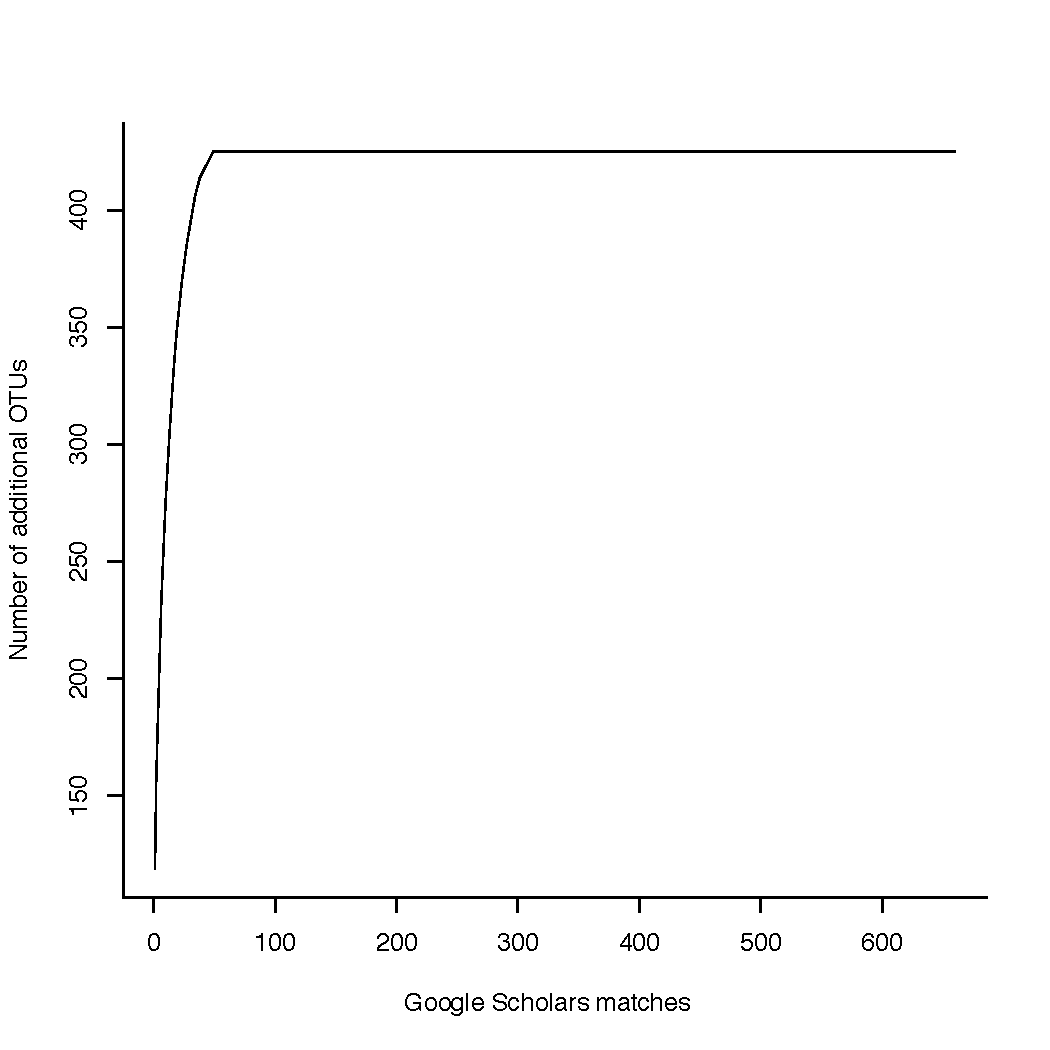
\includegraphics[width=1\textwidth]{Supp_figure_google_searches.pdf}
\caption{Google Scholar searches additional OTUs rarefaction curve. The x-axis represents the number of Google Scholar matches (papers, books or abstracts) and the y-axis represents the cumulative number of additional living OTUs for each Google Scholar match.}
\label{Supp_figure_google_searches}
\end{figure}

The list of all 286 downloaded matrices is available on \url{github.com/TGuillerme/Missing_living_mammals/tree/master/Data/Matrices}.
The matrices contained a total of 11010 operational taxonomic units (OTUs) of which 5228 were unique.
In this study, we refer to OTUs rather than species because the entries in the downloaded matrices were not standardised and ranged from specific individual specimen names (i.e. the name of a collection item) to the family-level.
Where possible, we considered OTUs at their lowest valid taxonomic level (i.e. species) but some OTUs were only valid at a higher taxonomic level (e.g. genus or family).
Therefore for some orders, we sampled more genera than species.

\subsection{Standardising the matrices}
We transformed all the non-NEXUS matrices (TNT, Word, Excel, JPEG) to NEXUS format manually.
We then cleaned the NEXUS matrices by removing any extra information (trees, continuous characters, morphological character descriptions, molecular data) to end up with NEXUS matrices containing only the discrete morphological data.
We then manually fixed the incorrectly-formatted binomial names (e.g. \textit{H. sapiens} became \textit{Homo sapiens}) using the abbreviation list in the relevant publications. 
All the standardised matrices are available on \url{github.com/TGuillerme/Missing_living_mammals/tree/master/Data/Matrices_binomial/Matrices}.

\subsection{Selecting the living OTUs}
We designated as ``living'' all OTUs that were either present in the phylogeny of \cite{bininda-emondsthe2007} or the taxonomy of \cite{wilson2005mammal}, and designated as ``fossil'' all OTUs that were present in the Paleobiology database (\url{paleobiodb.org/}).
For OTUs that did not appear in these three sources, we first decomposed the name (i.e. \textit{Homo sapiens} became \textit{Homo} and \textit{sapiens}) and tried to match the first element with a higher taxonomic level (family, genus etc.).
Any OTUs that still had no matches in the sources above were designated as non-applicable (NA; Figure ~\ref{Supp_figure_Taxonomic_algorithm}).
Non-applicable OTUs were either specimen IDs with no related taxon names (e.g. \textit{FMNHPR2081}), abbreviations that were not described in the associated paper (e.g. \textit{Ho.sap.}), non-mammals \textit{stricto-sensu} (e.g. \textit{Sinoconodon}), non standard taxonomic levels (e.g. \textit{Spalcotheriids}) invalid taxonomic designations (e.g. \textit{sp\_nov\_1} or \textit{Outgroup}) or typos (e.g. \textit{Hobo sapions}).

\begin{figure}[!htbp]
\centering
    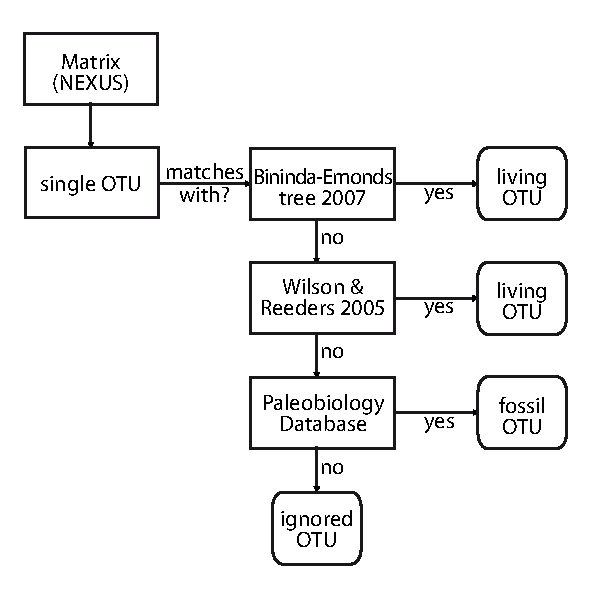
\includegraphics[width=1\textwidth]{Supp_figure_Taxonomic_algorithm.pdf}
\caption{Taxonomic matching algorithm used in this study. For each matrix, each operational taxonomic unit (OTU) is matched with the supertree from Fritz et al. 2009. If the OTU matches, then it is classified as living. Otherwise it is matched with the Wilson \& Reeder 2005 mammalian taxonomy. If the OTU matches, then it is classified as living. Otherwise it is matched with the Paleobiology database list of mammals. If the OTU matches, then it is classified as fossil. Otherwise it is ignored.}
\label{Supp_figure_Taxonomic_algorithm}
\end{figure}

\section{2 - Data collection reproducibility}
Every step of the analysis (apart from downloading and standardisation of the matrices) is entirely repeatable via GitHub (\url{github.com/TGuillerme/Missing_living_mammals}).

\newpage

\bibliographystyle{vancouver}
\bibliography{Supp_References}

\end{document}